\documentclass[sigconf]{acmart}
\usepackage{algorithm}
\usepackage{caption}
\usepackage{todonotes}
\usepackage{algorithmicx}
\usepackage[noend]{algpseudocode}

\newtheorem*{remark}{Remark}
\newtheorem*{note}{Note}

%%
%% \BibTeX command to typeset BibTeX logo in the docs
\AtBeginDocument{%
  \providecommand\BibTeX{{%
    \normalfont B\kern-0.5em{\scshape i\kern-0.25em b}\kern-0.8em\TeX}}}

%% Rights management information.  This information is sent to you
%% when you complete the rights form.  These commands have SAMPLE
%% values in them; it is your responsibility as an author to replace
%% the commands and values with those provided to you when you
%% complete the rights form.
\setcopyright{acmcopyright}
\copyrightyear{2018}
\acmYear{2018}
\acmDOI{10.1145/1122445.1122456}

%% These commands are for a PROCEEDINGS abstract or paper.
\acmConference[Woodstock '18]{Woodstock '18: ACM Symposium on Neural
  Gaze Detection}{June 03--05, 2018}{Woodstock, NY}
\acmBooktitle{Woodstock '18: ACM Symposium on Neural Gaze Detection,
  June 03--05, 2018, Woodstock, NY}
\acmPrice{15.00}
\acmISBN{978-1-4503-XXXX-X/18/06}


%%
%% Submission ID.
%% Use this when submitting an article to a sponsored event. You'll
%% receive a unique submission ID from the organizers
%% of the event, and this ID should be used as the parameter to this command.
%%\acmSubmissionID{123-A56-BU3}

%%
%% The majority of ACM publications use numbered citations and
%% references.  The command \citestyle{authoryear} switches to the
%% "author year" style.
%%
%% If you are preparing content for an event
%% sponsored by ACM SIGGRAPH, you must use the "author year" style of
%% citations and references.
%% Uncommenting
%% the next command will enable that style.
%%\citestyle{acmauthoryear}

%%
%% end of the preamble, start of the body of the document source.
\begin{document}

%%
%% The "title" command has an optional parameter,
%% allowing the author to define a "short title" to be used in page headers.
\title{Context-Free Path Queries, Planar Graphs and Friends}
 
%%
%% The "author" command and its associated commands are used to define
%% the authors and their affiliations.
%% Of note is the shared affiliation of the first two authors, and the
%% "authornote" and "authornotemark" commands
%% used to denote shared contribution to the research.

\author{Alexandra Istomina}
\affiliation{%
  \institution{Saint-Petersburg State University}
  \city{Saint-Petersburg}
  \country{Russia}
 }

\author{Alexandra Olemskaya}
\affiliation{%
  \institution{Inria Paris-Rocquencourt}
  \city{Rocquencourt}
  \country{France}
}

\author{Ekaterina Shemetova}
\affiliation{%
  \institution{Inria Paris-Rocquencourt}
  \city{Rocquencourt}
  \country{France}
}


\author{Semyon Grigorev}
\affiliation{%
 \institution{Rajiv Gandhi University}
 \streetaddress{Rono-Hills}
 \city{Doimukh}
 \state{Arunachal Pradesh}
 \country{India}}



%%
%% By default, the full list of authors will be used in the page
%% headers. Often, this list is too long, and will overlap
%% other information printed in the page headers. This command allows
%% the author to define a more concise list
%% of authors' names for this purpose.

%%
%% The abstract is a short summary of the work to be presented in the
%% article.
\begin{abstract}

Abstract is very abstract.

\end{abstract}

%%
%% The code below is generated by the tool at http://dl.acm.org/ccs.cfm.
%% Please copy and paste the code instead of the example below.
%%
\begin{CCSXML}
<ccs2012>
 <concept>
  <concept_id>10010520.10010553.10010562</concept_id>
  <concept_desc>Computer systems organization~Embedded systems</concept_desc>
  <concept_significance>500</concept_significance>
 </concept>
 <concept>
  <concept_id>10010520.10010575.10010755</concept_id>
  <concept_desc>Computer systems organization~Redundancy</concept_desc>
  <concept_significance>300</concept_significance>
 </concept>
 <concept>
  <concept_id>10010520.10010553.10010554</concept_id>
  <concept_desc>Computer systems organization~Robotics</concept_desc>
  <concept_significance>100</concept_significance>
 </concept>
 <concept>
  <concept_id>10003033.10003083.10003095</concept_id>
  <concept_desc>Networks~Network reliability</concept_desc>
  <concept_significance>100</concept_significance>
 </concept>
</ccs2012>
\end{CCSXML}

\ccsdesc[500]{Computer systems organization~Embedded systems}
\ccsdesc[300]{Computer systems organization~Redundancy}
\ccsdesc{Computer systems organization~Robotics}
\ccsdesc[100]{Networks~Network reliability}

%%
%% Keywords. The author(s) should pick words that accurately describe
%% the work being presented. Separate the keywords with commas.
\keywords{datasets, neural networks, gaze detection, text tagging}


%%
%% This command processes the author and affiliation and title
%% information and builds the first part of the formatted document.
\maketitle
\input{introduction.tex}
\input{preliminaries.tex}
\input{planar.tex}
\section{CFPQ on undirected graphs}

\subsection{Motivation}

The bottleneck of the Tensor-based algorithm is computing Incremental transitive closure, which cannot be solved in subcubic 
% (that is, $\mathcal{O}(n^{3 - \varepsilon})$) 
time.

So to speed up the algorithm, it is necessary to modify this particular part somehow.

We decided to relax the task and find incremental transitive closure, not in a directed graph, but an undirected one. The motivation behind this decision is simple: the problem of Incremental transitive closure in an undirected graph is easier than directed and can be solved in less running time.

\subsection{Definitions} ~

\definecolor{dkgreen}{rgb}{0,0.6,0}

\textit{\color{dkgreen}{\# define}} $G$~-- input grammar

\textit{\color{dkgreen}{\# define}} $q_i$~--- grammar states

\textit{\color{dkgreen}{\# define}} $\mathcal{G}$~--- input graph

\textit{\color{dkgreen}{\# define}} $u, v$~--- graph vertices

\subsection{Algorithm}

% At first, we assume, that each RSM box (of given grammar) is acyclic (if not, we can replace cycles with recursive call (how? {\color{red}{TODO}}))
% Then we can topologically sort every box (so that for every arc $q_i \rightarrow v \Leftrightarrow u < v$).


We use two data structures: queue $Q$, storing edges, that should be added, but have not been yet, and Disjoint Set $D$, maintaining components in Kronecker product graph.

Firstly, we add all arcs from initial Kronecker product into $Q$ and then start to iterate over it. At each step we take next arc from queue and join corresponding sets in $D$. If they are in differents sets and adding the edge leads to appearance of new path $(q_s, u) \rightsquigarrow (q_f, v)$ from start to final terminal of some box $S$, we add new arc form $u$ to $v$ labeled with $S$. After that we add this arc into Kronecker product: we iterate over all arcs $q_i \rightarrow q_j$ in grammar $G$ labeled with $S$ and add new edge $(q_i, u) \rightarrow (q_j, v)$ into $Q$. 

\begin{algorithm}[H]
    \floatname{algorithm}{Listing}
    \begin{algorithmic}[1]
    \caption{Undirected Kronecker product based CFPQ}
    \label{alg:UndirectodTensor}
    \Function{undirectedContextFreePathQuerying}{G, $\mathcal{G}$}
        % Input data preparation
        \State{$R \gets$ Recursive automata for $G$}
        \State{$M_1 \gets$ Adjacency matrix for $R$}
        \State{$M_2 \gets$ Adjacency matrix for $\mathcal{G}$}
        \State{$M_3 \gets M_1 \otimes M_2$}
        \State{$Q \gets$ Empty Queue}
        \State{$D \gets$ Empty Disjoint Set}
        \State{$n \gets$ dim($M_3)$}
        \For{$i \in 0..n-1$}
            \State{$D.MakeSet(i)$}
            \Comment{Create empty set for every element in Kronecker product}
        \EndFor
        \For{$x \in 0..n-1$}
           \For{$y \in 0..n-1$}
                \If{$M_3[x,y]$}
                    \State{$Q.Add(x, y)$}
                    \Comment{Add initial edges}
                \EndIf
           \EndFor
        \EndFor
        \While{$Q$ is not empty}
            \State{$(x, y) \gets Q.Pop()$}
            \For {$(q_s, u) \in D.Find(x).GetInitialStates()$}
                \For {$(q_f, v) \in D.Find(y).GetFinalStates()$}
                    \State{$S \gets G.GetLabelByState(q_s)$}
                    \For{$(q_i, q_j) \in GetEdgesByLabel(S)$}
                        \State{$Q.Push((q_i, u), (q_j, v))$}
                        \State{$M_3[(q_i, u), (q_j, v)] \gets 1$}
                        \Comment{Add new edges}
                    \EndFor
               \EndFor
            \EndFor
            \State{$D.Merge(x, y)$}
        \EndWhile
    \State \Return $M_3$
    \EndFunction
    \end{algorithmic}
\end{algorithm}

To find new paths from start to final terminal quickly, we store for every set in $D$ all initial and final states in it. To get this information we use supporting methods $GetInitialStates()$ and $GetFinalStates()$. To get RSM box label by state id we use supporting method $GetLabelByState()$. To get all edges in grammar labeled with $S$ we use supporting method $GetEdgesByLabel()$. 

{\color{red}{TODO}}: rewrite in other notations

{\color{red}{TODO}}: write about dealing with eps-transitions.

\subsection{Complexity}

{\color{red}{TODO}}

\subsection{Bidirected graphs}

\begin{definition}

{\bf Bidirected Graphs.}

A $\Sigma_k$ labeled graph $G = (V, E)$ is called bidirected if for every pair of nodes $u, v \in V$ for all $1 \le i \le k$ we have that $(u, v, \alpha_i) \in E$ iff $(v, u, \overline{\alpha_i}) \in E$. 
Informally, the edge relation is symmetric, and the labels of symmetric edges are complimentary wrt to opening and closing parenthesis. 
\end{definition}

\begin{remark} \label{r1}
    For bidirected graphs the Dyck-reachability relation forms an equivalence, i.e., for all bidirected graphs $G$, for every pair of nodes $u$m $v$, we have that $v$ is Dyck-reachable from $u$ iff $u$ is Dyck-reachable from $v$.
\end{remark}

\begin{note}
    Dyck language RSM-grammar box (there is only one).
    
    \begin{figure}[H]
        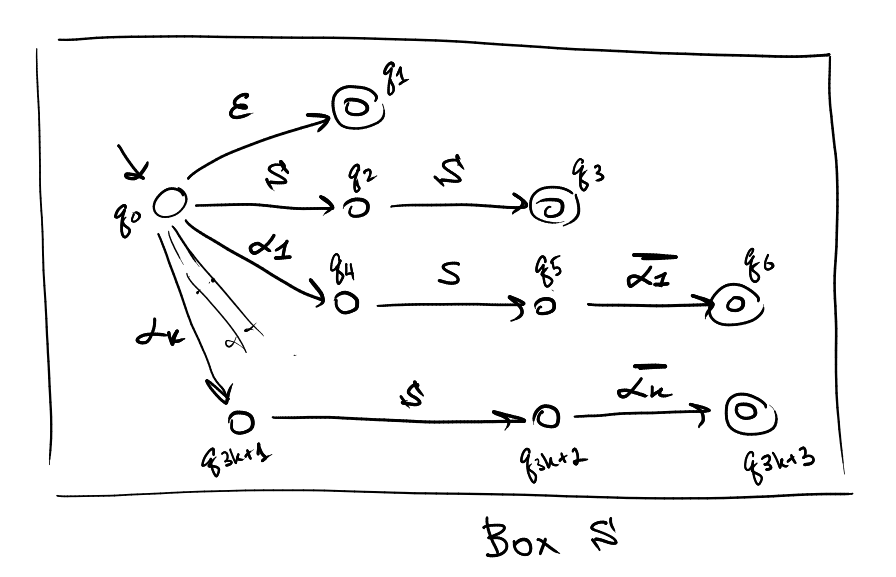
\includegraphics[width=\linewidth]{img/dyck_box.png}
    \end{figure}
\end{note}


\begin{theorem}
The Algorithm \ref{alg:UndirectodTensor} works correctly on bidirected graphs and Dyck grammars.
\end{theorem}
\begin{proof}

We only need to prove, that for every pair $u, v \in V(\mathcal{G})$ there is a path $(q_s, u) \rightsquigarrow (q_{f_i}, v)$ in ({\bf directed}) Kronecker product $G \otimes \mathcal{G}$ 
iff 
there is such path $(q_s, u) \rightsquigarrow (q_{f_j}, v)$ in an {\bf undirected} product (there $q_s$ is the initial state and $q_{f_i}, q_{f_j}$ are some final states of $G$ respectively).

$\Rightarrow$ 

Obviously (if $(q_{f}, v)$ is reachable from $(q_{s}, u)$ by directed edges, it is all the more reachable by undirected edges).

$\Leftarrow$

At first, note that the Kronecker product $G \otimes \mathcal{G}$ forms some kind of a layered structure~--- $i$-th layer consists of vertices $(q_i, v)$, where $q_i$ is $i$-th RSM state. Because RSM is topologically sorted ({\color{red}{TODO}}), every edge $(q_i, u) \rightarrow (q_j, v)$ goes forward.

We will call path \textit{simple} if it visits every layer no more than once.

We prove the claim by induction on the $l$ (path length).

Clearly the result is true for $l \le 3$, because the only way to achive final vertex in $1, 2$ or $3$ edges is by a simple vertical path (which exists in the original graph too).

Otherwise (if $l \ge 4$), path is not simple. 

Consider the first flex point of the path, that is the vertex $(q_i, v)$ such that edges $(q_j, u) \rightarrow (q_i, v)$ and $(q_i, v) \rightarrow (q_k, w)$ are in the path and $j, k \le i$ (so, the path is convex at this point).

Looking at the grammar graph we can notice, that every state has indegree $\le 1$. So at the flex point there are actually two same-labeled edges (that is, $j = k$). 

There can be three different types of labels on those edges:

\begin{itemize}
    \item $\alpha_l$-label

        \textit{path: $(q_0, u) \rightarrow (q_i, v) \rightarrow (q_0, w) \rightarrow \dots \rightarrow (q_f, z)$.}

        Since $\alpha_l$-labeled edges could only be added on the initialization stage, 
        graph $\mathcal{G}$ contains edges $u \xrightarrow{\alpha_l} v$ and $w \xrightarrow{\alpha_l} v$. Notice, that cause $\mathcal{G}$ is bidirected, it also has to contain edges $v \xrightarrow{\overline{\alpha_l}} u$ and $v \xrightarrow{\overline{\alpha_l}} w$.

        Now we can notice, that $w$ is Dyck-reachable (by the path $\alpha_l \overline{\alpha_l}$) from $u$, so there is an $S$-labeled edge from $u$ to $w$. We can also conclude, that (by induction) there is a directed path from $(q_0, w)$ to $(q_f, z)$ (there $z$ is the end of the path and $q_f$ is some final state of $G$), so there is an $S$-labeled edge from $w$ to $z$. 

        Using this two observation we can construct a directed path from $u$ to $z$: $u \xrightarrow{S} w \xrightarrow{S} z$. 
    \item $S$-label

        \textit{path: $(q_0, a) \rightarrow \dots \rightarrow (q_j, u) \rightarrow (q_i, v) \rightarrow (q_j, w) \rightarrow \dots \rightarrow (q_f, z)$.}

        $\mathcal{G}$ contains $S$-labeled edges $u \xrightarrow{S} v$ and $w \xrightarrow{S} v$. Since $\mathcal{G}$ is bidirected, then by \ref{r1} $v \xrightarrow{S} u$ and $v \xrightarrow{S} w$. Combining $u \xrightarrow{S} v$ and $v \xrightarrow{S} w$ we get that $u \xrightarrow{S} w$. 

        No we want to sort of contract this edge, joining $u$ and $w$ (on the $j$-th level). Then we can get (by induction hypothesis) the directed path from $(q_0, a) \rightsquigarrow (q_f, z)$. If new path does not contain joined $uw$ vertex, then that's the answer. Otherwise we can split this vertex back, inserting between $u$ and $w$ the $S$-labeled path (that one, from $u \xrightarrow{S} w$ edge). We can do it, because the both of these paths form correctly matched parenthesis ({\color{red}{TODO}}: we can prove this using stack-based checking algorithm).

        \textit{Two other cases can be proved the same way, but I find it a little dishonest}

    \item $\overline{\alpha_l}$-label

        \textit{path: $(q_0, a) \rightarrow \dots \rightarrow (q_j, u) \rightarrow (q_f, v) \rightarrow (q_j, w) \rightarrow \dots \rightarrow (q_f, z)$.}

        Since $\alpha_l$-labeled edges could only be added on the initialization stage, 
        graph $\mathcal{G}$ contains edges $u \xrightarrow{\overline{\alpha_l}} v$ and $w \xrightarrow{\overline{\alpha_l}} v$. Notice, that cause $\mathcal{G}$ is bidirected, it also has to contain edges $v \xrightarrow{\alpha_l} u$ and $v \xrightarrow{\alpha_l} w$.

        By induction, we get that $a \xrightarrow{S} v$. Now we will construct a second part of the path: $(q_0, v) \xrightarrow{\alpha_l} (q_{j-1}, w) \xrightarrow{S} (q_j, w) \rightsquigarrow (q_f, z)$ ($q_{j-1}, w) \xrightarrow{S} (q_j, w)$ ~--- initial $S$-loop). By induction, we have directed simple version of this path, so $v \xrightarrow{S} z$. 

        Combining this two paths ($a \xrightarrow{S} v$ and $v \xrightarrow{S} z$) we get $a \xrightarrow{SS} z \Rightarrow a \xrightarrow{S} z$~--- desired path.
        
    \begin{figure}[H]
        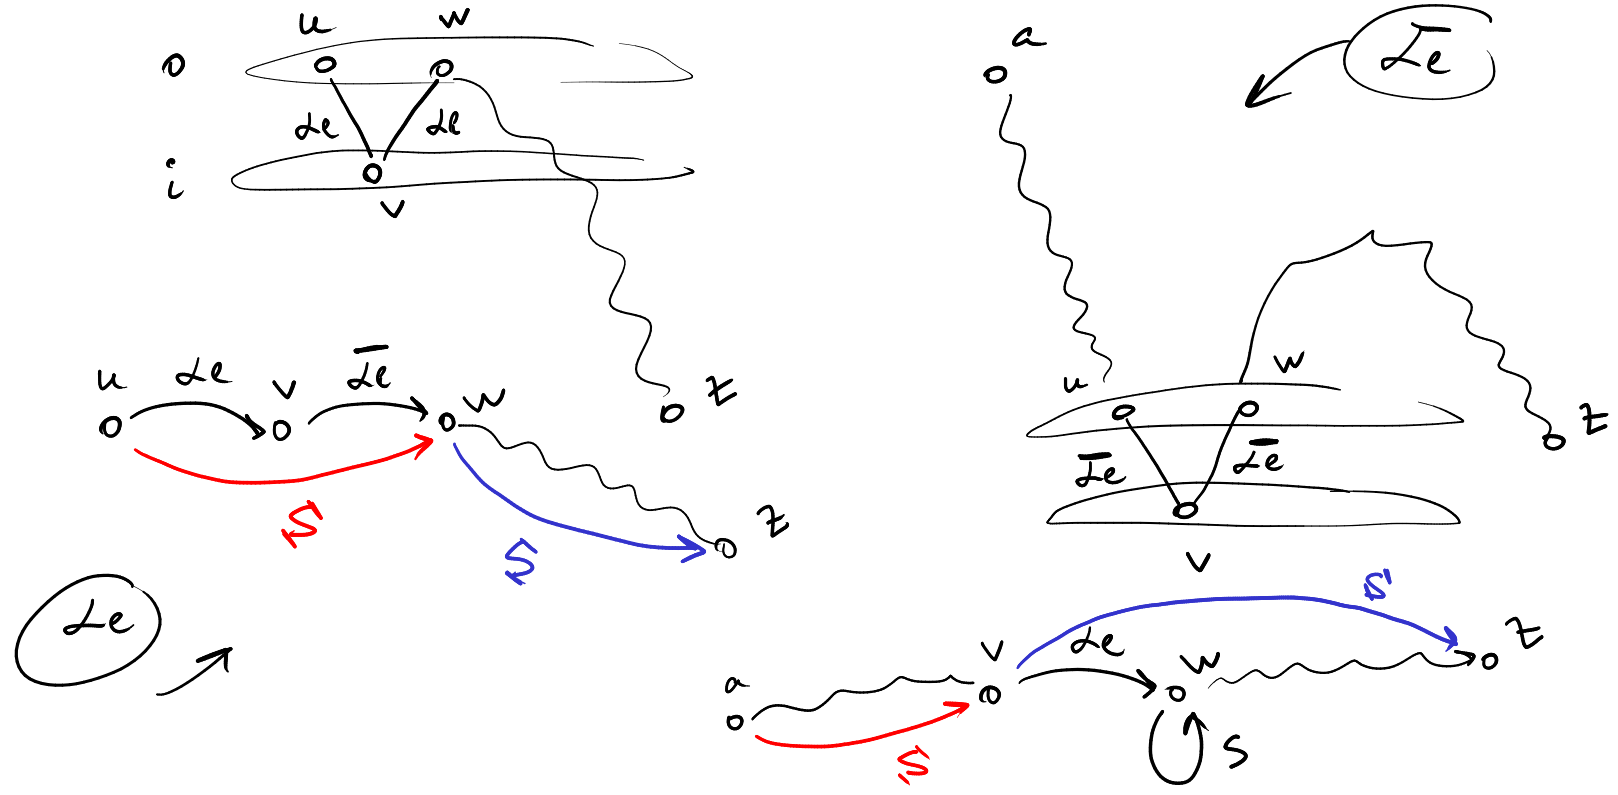
\includegraphics[width=\linewidth]{img/th_proof_img.png}
    \end{figure}
\end{itemize}

\end{proof}


\subsection{MYCOPKA}

bidirected guys \cite{10.1145/2491956.2462159}

resalt about Dyck-reachability components \cite{10.1145/2499370.2462159}
\input{conclusion.tex}



%%
%% The next two lines define the bibliography style to be used, and
%% the bibliography file.
\bibliographystyle{ACM-Reference-Format}
\bibliography{references}

\end{document}
\endinput
%%
%% End of file `sample-sigconf.tex'.
